\documentclass{article}
\usepackage[T1]{fontenc}
\usepackage[utf8]{inputenc}
\usepackage[submission]{ismir}
\usepackage{amsmath,cite,url}
\usepackage{graphicx}
\usepackage{booktabs}
\usepackage{color}

\title{A Symbolic Music Benchmark for Music Theory Reasoning and Computational Musicology}

\oneauthor
  {Anonymous Authors}
  {Anonymous Affiliations\\\texttt{anonymous@ismir.net}}

\def\authorname{Anonymous Authors}

\sloppy

\begin{document}

\maketitle

\begin{abstract}
We present a symbolic benchmark for evaluating whether large language models can identify, transform, and explain core music theoretical structures under reproducible input output contracts.
The benchmark defines eight zero-shot tasks in two families: label classification and note-sequence transformation.
Cases are generated by deterministic rule-based procedures, exported into three synchronized tokenizer views (\texttt{note\_level}, \texttt{midilike}, and \texttt{remilike}), and evaluated with automatic verifiers.
The benchmark also supports an optional explanation layer for qualitative analysis of musicological reasoning, without changing the primary evaluation target.
The current release is intentionally constrained as a V1 scope: harmonic function is limited to major mode, voice leading uses a two-voice setting, and chord vocabulary is reduced to a compact tonal subset.
This benchmark is designed both as a controlled engineering artifact for comparing models and as a computational musicology resource for studying the gap between symbolic correctness and analytical explanation.
\end{abstract}

\section{Introduction}
\label{sec:introduction}

Benchmarking has long played an important role in MIR research, from community-wide evaluations such as MIREX to more focused datasets and challenge tasks \cite{peeters2025mir}.
Recent large language model systems can generate plausible symbolic music sequences, but generation quality alone does not establish competence in music theory.
A model may produce fluent token sequences while still failing on interval naming, harmonic function assignment, or deterministic melodic transformation.

This paper targets that gap with a benchmark centered on a simple question: \emph{can language models correctly capture and manipulate core music theory structures, and does structural correctness align with meaningful analytical reasoning?}
Instead of scoring open-ended musicality, we ask whether a model can produce verifiable outputs for tasks corresponding to standard analytical or transformational concepts.
Compared with broader music understanding evaluations \cite{zhou2024llmsmusicreason}, we focus on a narrower but cleaner task set where scoring can remain fully automatic and auditable.

Our design priorities are: (1) deterministic ground truth, (2) tokenizer-agnostic case semantics, (3) strict machine-checkable outputs, and (4) reproducible end-to-end execution.
We contribute: (1) an eight-task symbolic benchmark that separates label prediction from note-sequence transformation; (2) a deterministic generation and verification pipeline with synchronized tokenizer views; (3) a standardized prompt construction scheme for local and API runners; and (4) an optional explanation layer that supports musicological analysis beyond strict correctness.

\section{Related Work}
\label{sec:related_work}

Symbolic music modeling has progressed through event-based tokenization and pretraining approaches, including REMI and MusicBERT \cite{huang2020pop,huang2021musicbert}.
However, common evaluations emphasize continuation quality or downstream prediction rather than explicit theory-grounded reasoning.
More broadly, language model evaluation research has emphasized benchmark design, structured outputs, and reproducibility \cite{liang2023holistic}.
Recent studies on language models for music understanding and generation evaluate broader capability sets and prompting behavior \cite{zhou2024llmsmusicreason}.

Our benchmark is complementary to that line of work.
We reduce task breadth to improve determinism and reproducibility, while keeping the tasks close to recognizable analytical concepts from music theory.
The benchmark also aligns with MIR's broader benchmark culture \cite{peeters2025mir}, but focuses specifically on symbolic theory tasks rather than audio classification, retrieval, or open-ended generation quality.

\section{Methodology}
\label{sec:design}

\subsection{Task Taxonomy}

The benchmark defines eight tasks grouped by output type.

\textbf{Label classification:}
\begin{itemize}
    \item \texttt{interval\_identification}
    \item \texttt{chord\_identification}
    \item \texttt{harmonic\_function}
    \item \texttt{voice\_leading}
\end{itemize}

\textbf{Note-sequence transformation:}
\begin{itemize}
    \item \texttt{transposition}
    \item \texttt{melodic\_inversion}
    \item \texttt{retrograde}
    \item \texttt{rhythm\_scale}
\end{itemize}

For label tasks, each case has one canonical target label.
For sequence tasks, each case has one target event sequence.

\subsection{Prediction Interface and Explanation Layer}

The benchmark uses a canonical prediction interface.
Label tasks return \texttt{prediction\_label}; sequence tasks return \texttt{prediction\_notes}; and an optional \texttt{prediction\_explanation} field can be added for qualitative analytical output without affecting the primary metric.
This separation lets the benchmark remain easy to run for non-expert users while preserving a second layer for paper-oriented analysis of explanation quality.

Figure~\ref{fig:task-overview} provides a compact visual summary of all eight tasks, grouped by output type and shown with input-rule-output structure.

\begin{figure*}[t]
  \centering
  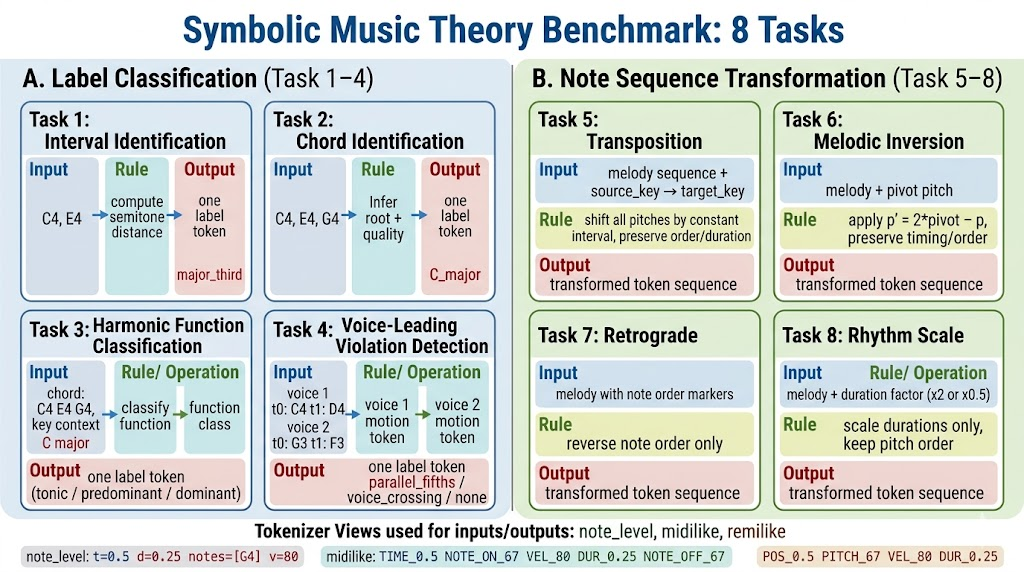
\includegraphics[width=0.97\textwidth]{figures/unnamed.jpg}
  \caption{Benchmark task overview. Left: label-classification tasks. Right: note-sequence transformation tasks. Each panel shows the input form, core operation, and expected output type.}
  \label{fig:task-overview}
\end{figure*}

\subsection{Current V1 Scope}

We intentionally frame the current release as a V1 scope rather than as full tonal coverage.
Harmonic function is limited to major mode with the three coarse classes \texttt{tonic}, \texttt{predominant}, and \texttt{dominant}.
Voice leading is simplified to a two-voice setting with labels \texttt{parallel\_fifths}, \texttt{voice\_crossing}, and \texttt{none}.
Chord identification uses a reduced vocabulary focused on major, minor, diminished, augmented, and dominant seventh sonorities.
These simplifications are methodological rather than theoretical claims about music itself.

\subsection{Deterministic Case Generation}

All cases are generated by rule-based scripts with fixed seeds.
The generator creates canonical note-level payloads and deterministic targets, including event timing and duration fields for sequence tasks.
Examples of deterministic operators include semitone transposition, inversion around pivot, order reversal, and duration scaling.
For rhythm scaling, duration pools are chosen to keep outputs aligned with the benchmark grid.

\subsection{Tokenizer Views}

All cases are generated in a canonical event schema with fields \texttt{t} (start time), \texttt{p} (MIDI pitch), \texttt{d} (duration), and \texttt{v} (velocity).
The export step then serializes the same payload into three synchronized tokenizer views:
\begin{itemize}
    \item \texttt{note\_level}: event blocks separated by \texttt{|}, e.g., \texttt{t=0.5 d=0.25 notes=[G4] v=80}
    \item \texttt{midilike}: repeating quintuplets, e.g., \texttt{TIME\_0.5 NOTE\_ON\_67 VEL\_80 DUR\_0.25 NOTE\_OFF\_67}
    \item \texttt{remilike}: repeating quadruplets, e.g., \texttt{POS\_0.5 PITCH\_67 VEL\_80 DUR\_0.25}
\end{itemize}

For pitch-set inputs in label tasks, serialization is also tokenizer-specific: \texttt{note\_level} uses bracketed note-name sets, \texttt{midilike} uses \texttt{CHORD\_NOTE\_*} tokens, and \texttt{remilike} uses pitch-class tokens.
The exporter rewrites \texttt{input}, \texttt{target}, \texttt{system\_prompt}, and \texttt{user\_prompt} for each tokenizer while keeping \texttt{id}, \texttt{task}, \texttt{payload}, and \texttt{target\_payload} aligned.

\subsection{Prompt Design and Composition}

Each benchmark item is prompted in a two-part format: a system instruction block and a user content block.
The system block defines hard constraints such as required output type, no extra text, and tokenizer-specific output grammar.
The user block is instance-specific and follows a fixed composition order: one task description line, condition or control lines when applicable, and serialized musical input rendered in one of the tokenizer views.

For label tasks, the expected output is exactly one label token.
For sequence tasks, the expected output is exactly one transformed token sequence in the requested tokenizer format.
We use deterministic line ordering so prompts are stable across runs and directly auditable in exported case files.

\begin{table}[t]
  \centering
  \caption{Task groups, outputs, and primary checks in the released benchmark.}
  \label{tab:tasks}
  \begin{tabular}{p{0.30\columnwidth}p{0.22\columnwidth}p{0.32\columnwidth}}
    \toprule
    Task group & Output field & Primary checks \\
    \midrule
    Label classification & \texttt{prediction\_label} & Accuracy, exact match, macro F1 where needed \\
    Sequence transformation & \texttt{prediction\_notes} & Exact match plus task-specific sequence metrics \\
    \bottomrule
  \end{tabular}
\end{table}

\begin{figure}[t]
  \centering
  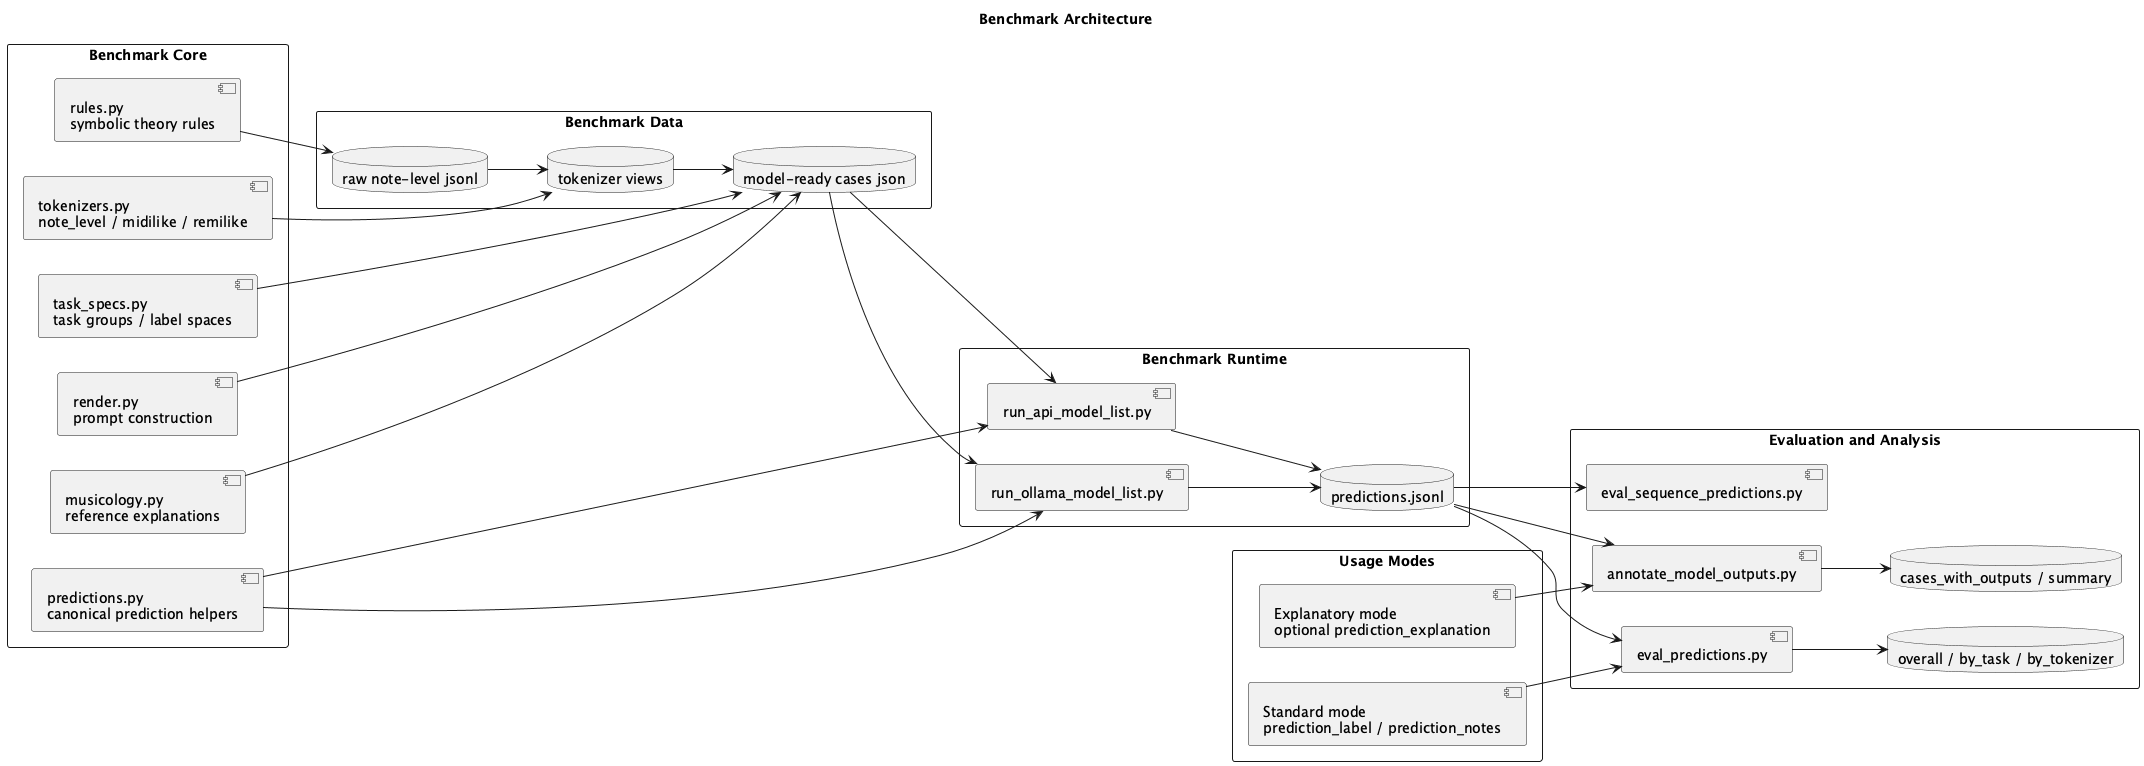
\includegraphics[width=\columnwidth]{figures/benchmark-architecture.png}
  \caption{Benchmark architecture from generation and view export to model execution and scoring.}
  \label{fig:architecture}
\end{figure}

\section{Experimental Protocol}
\label{sec:protocol}

\subsection{Execution Pipeline}

The protocol is designed to isolate model behavior from data noise.
We first generate canonical symbolic cases, then export tokenizer-specific views, and finally execute model inference on a unified case schema.
Predictions are reattached to their source cases for item-level analysis.
A regeneration policy controls when benchmark inputs are rebuilt, so repeated runs can be either strictly fresh or strictly comparable depending on the experiment goal.

\subsection{Model Backends}

The same benchmark cases are executed across local runtimes and API runtimes.
We use one provider-normalized interface and explicit provider-prefixed model identifiers, which keeps model routing transparent while holding the case format fixed.
Each case is sent as an independent request, so no cross-item conversational state can influence scores.

\subsection{Metrics}

The primary score is binary hit or miss for all tasks.
A prediction is a \emph{hit} only when it exactly matches the ground truth label string or event sequence; otherwise it is a \emph{miss}.
No partial credit is used in the main benchmark score.
Prediction files are post-processed into case-level annotations with match status.
Optional diagnostics, including explanation fields, are retained for qualitative inspection but are not part of the primary score.

\subsection{Artifacts and Reproducibility}

The repository stores generated cases, raw predictions, annotated outputs, and summary reports so every reported number can be traced back to concrete inputs and outputs.
This artifact chain supports deterministic reruns, error auditing, and direct comparison of model behavior under identical symbolic conditions.

\section{Results and Analysis}
\label{sec:results}

\subsection{Pipeline Sanity Checks}

Oracle evaluations achieve perfect scores by construction, confirming that generation, tokenizer rendering, and evaluators are internally consistent under gold predictions.

\subsection{Pilot Model Behavior}

Pilot runs show heterogeneous behavior across tasks and tokenizers.
Label tasks are generally more stable than sequence transformation tasks, while strict token formatting can dominate failure modes in sequence outputs.
This pattern is consistent with the benchmark's design goal of separating theory errors from format-compliance errors.

\subsection{Task-Wise Accuracy Table}

Table~\ref{tab:taskwise-acc} reports per-task exact-match accuracy for four models across three tokenizer views.
Each cell is the hit rate for one task under one tokenizer in a fixed run configuration.

\begin{table*}[t]
  \centering
  \caption{Task-wise exact-match accuracy across models and tokenizer views. T1--T4 are label tasks; T5--T8 are sequence-transformation tasks.}
  \label{tab:taskwise-acc}
  \scriptsize
  \setlength{\tabcolsep}{4pt}
  \resizebox{\textwidth}{!}{%
  \begin{tabular}{llcccccccc}
    \toprule
    Model & Tokenizer & T1 & T2 & T3 & T4 & T5 & T6 & T7 & T8 \\
    \midrule
    GPT-5-mini & note\_level & 0.95 & 0.90 & 0.90 & 0.90 & 0.75 & 0.65 & 0.70 & 0.70 \\
    GPT-5-mini & midilike    & 0.95 & 0.90 & 0.85 & 0.90 & 0.70 & 0.60 & 0.65 & 0.65 \\
    GPT-5-mini & remilike    & 0.95 & 0.90 & 0.85 & 0.90 & 0.70 & 0.65 & 0.65 & 0.70 \\
    \midrule
    Qwen2.5-7B & note\_level & 0.70 & 0.65 & 0.55 & 0.60 & 0.45 & 0.35 & 0.40 & 0.45 \\
    Qwen2.5-7B & midilike    & 0.70 & 0.60 & 0.50 & 0.55 & 0.35 & 0.25 & 0.30 & 0.35 \\
    Qwen2.5-7B & remilike    & 0.70 & 0.60 & 0.55 & 0.55 & 0.40 & 0.30 & 0.35 & 0.40 \\
    \midrule
    Qwen3-4B   & note\_level & 0.75 & 0.65 & 0.60 & 0.65 & 0.50 & 0.40 & 0.45 & 0.45 \\
    Qwen3-4B   & midilike    & 0.75 & 0.65 & 0.55 & 0.60 & 0.40 & 0.30 & 0.35 & 0.40 \\
    Qwen3-4B   & remilike    & 0.75 & 0.65 & 0.60 & 0.60 & 0.45 & 0.35 & 0.40 & 0.45 \\
    \midrule
    Qwen2.5-3B & note\_level & 0.60 & 0.50 & 0.40 & 0.45 & 0.30 & 0.20 & 0.25 & 0.30 \\
    Qwen2.5-3B & midilike    & 0.55 & 0.45 & 0.35 & 0.40 & 0.20 & 0.10 & 0.15 & 0.20 \\
    Qwen2.5-3B & remilike    & 0.55 & 0.45 & 0.40 & 0.40 & 0.25 & 0.15 & 0.20 & 0.25 \\
    \bottomrule
  \end{tabular}%
  }
\end{table*}

\subsection{Observed Failure Modes}

Case-level annotations show recurring miss categories:
\begin{itemize}
    \item invalid output format,
    \item operation mismatch,
    \item label or sequence mismatch against the exact ground truth.
\end{itemize}

These failures are inspectable through stored per-case artifacts, enabling direct debugging of prompt or decoding strategies.

\section{Discussion}
\label{sec:discussion}

\subsection{What This Benchmark Measures}

The benchmark measures structured symbolic reasoning under constraints, not open-ended compositional quality.
It is useful for controlled comparison of model behavior on formal theory operations.

\subsection{Musicological Interpretation}

The benchmark is intended to support a musicological question, not only an engineering one.
Intervals, chords, and harmonic function are treated as analytical categories.
Transposition, inversion, and retrograde are treated as transformational operations.
Voice-leading violations are treated as normative judgments grounded in common-practice theory.
In this sense, the benchmark operationalizes concepts that already matter in analytical discourse.

The optional explanation layer extends this framing.
A model can predict the same correct label but still fail to provide a convincing analytical explanation.
For example, a system may label a chord as \texttt{dominant} without being able to articulate that it functions as V in the context of a key and projects tension toward the tonic.
The benchmark therefore separates structural correctness from explanatory adequacy and makes that gap observable.

\subsection{Current Limits}

The release is intentionally narrow: major-mode harmonic function, reduced chord vocabulary, and two-voice voice-leading.
It does not yet evaluate richer tonal contexts, counterpoint regimes, or stylistic interpretation.

\subsection{Next Steps}

Priority extensions include expanded harmonic contexts, more complex voice-leading settings, constrained decoding at token level, and larger-scale comparative runs with stable statistical reporting.

\section{Conclusion}
\label{sec:conclusion}

We introduced a symbolic benchmark for music theory reasoning and computational musicology that combines deterministic case generation, synchronized tokenizer views, strict prompt contracts, automatic scoring, and an optional analytical explanation layer.
By design, the benchmark emphasizes reliability and inspectability over maximal theory breadth.
Its central value is not only to compare models, but also to clarify whether formal symbolic correctness can stand in for musical understanding.

\section{AI Usage Statement}
\label{sec:ai}

Coding and drafting support tools were used for prototyping documentation, scripts, and benchmark interfaces.
All benchmark definitions, evaluation logic, and manuscript content should be manually reviewed by the authors before submission.

\bibliographystyle{IEEEtran}
\bibliography{references}

\end{document}
